\documentclass{chi-ext}
% See http://personales.upv.es/luileito/chiext/

\usepackage{tikz}
\usepackage{verbatim}
%\usepackage[active,tightpage]{preview}
%\PreviewEnvironment{tikzpicture}

\copyrightinfo{
  Copyright is held by the author/owner(s).\\
  \emph{MobileHCI 2014}, September 23-26 2014, Toronto, Canada.\\
  ACM 978-1-XXXX-XXXX-X/XX/XX.\\
}

\title{Wearable Haptic Gaming Using Vibrotactile Arrays}

\numberofauthors{5}
% Notice how author names are alternately typesetted to appear ordered in 2-column format;
% i.e., the first 4 authors on the first column and the other 4 authors on the second column.
% Actually, it's up to you to strictly adhere to this author notation.
\author{
  \alignauthor{
  	\textbf{Adam Tindale}\\
  	\affaddr{OCAD University}\\
  	\affaddr{Toronto, ON M5T 1W1 Canada}\\
  	\email{atindale@faculty.ocadu.ca}
  }\alignauthor{
  	\textbf{Jessica Peter}\\
  	\affaddr{OCAD University}\\
  	\affaddr{Toronto, ON M5T 1W1 Canada}\\
  	\email{jp11jg@student.ocadu.ca}
  } 
    \vfil
  \alignauthor{
  	\textbf{Michael Cumming}\\
  	\affaddr{OCAD University}\\
  	\affaddr{Toronto, ON M5T 1W1 Canada}\\
  	\email{mcumming@ocadu.ca}
  }\alignauthor{
  	\textbf{Sara Diamond}\\
  	\affaddr{OCAD University}\\
  	\affaddr{Toronto, ON M5T 1W1 Canada}\\
  	\email{sdiamond@ocadu.ca}
  }
    \vfil
    \alignauthor{
  	\textbf{Hudson Pridham}\\
  	\affaddr{OCAD University}\\
  	\affaddr{Toronto, ON M5T 1W1 Canada}\\
  	\email{hp12pk@student.ocadu.ca}
  } 
}

% Paper metadata (use plain text, for PDF inclusion and later re-using, if desired)
\def\plaintitle{Wearable Haptic Gaming Using Vibrotactile Arrays}
\def\plainauthor{Adam Tindale}
\def\plainkeywords{haptic gaming, vibrotactile arrays, wearable devices, multi-sensory}
\def\plaingeneralterms{Wearable Gaming, Vibrotactile display, Wrist}

\hypersetup{
  % Your metadata go here
  pdftitle={\plaintitle},
  pdfauthor={\plainauthor},  
  pdfkeywords={\plainkeywords},
  pdfsubject={\plaingeneralterms},
  % Quick access to color overriding:
  citecolor=black,
  linkcolor=blue,
  menucolor=black,
  urlcolor=blue,
}

\usepackage{graphicx}   % for EPS use the graphics package instead
\usepackage{balance}    % useful for balancing the last columns
\usepackage{bibspacing} % save vertical space in references
\usepackage{paralist}
\usetikzlibrary{shapes,arrows}

\begin{document}

\maketitle

\begin{abstract}
%Simple, wearable devices are a promising way of encouraging participation with those who consume, and contribute to, media. 

%In this paper we describe a series of demo experiences focusing on the communication of information through low resolution vibrotactile and LED displays. The intended purpose for this exploration is to add simple visual and vibro-tactile patterning to wearable devices intended for children aged 8-12. These patterns add sensory interest to these devices and convey useful information about device dynamics and expected user interactions. 

%Framing the article around game controllers might be problematic since we do not return to this concept, nor do we address portable game devices or smart phones. Some phrasing, such as "and which the user would tend to find enjoyable and engaging even if they were not participating in a mobile game" suggests that the wearable can also be a controller, which it can't. Reframed regarding wearable tech for children w/ simple interaction as response to price demands and lack of smartphone integration.
%The recent launch of products such as Google Glass and the Pebble Smartwatch indicate a growing public interest in wearable personal electronics. However, outside of physical activity monitors and GPS trackers aimed at parents, few products are aimed towards younger users. In this paper, we explore techniques for designing wearable game devices for children aged 8-12. We describe a series of demo experiences which use simple visual and vibrotactile patterning to which add sensory interest to gameplay as well as convey useful information about game dynamics.

In this paper we describe the design process of expanding vibrotactile displays from single channels devices to multichannel vibrotactile displays. The purpose for this exploration is to add simple, interactive visual and vibro-tactile patterning with button arrays to wearable gaming devices intended for young children. In order to facilitate movement we have created numerous prototypes to examine the affordances and limitations of a circular pattern of tactors.

\end{abstract}

\keywords{\plainkeywords}

\category{H.5.2}{Information interfaces and presentation (e.g., HCI)}{User Interfaces}. 

\terms{\plaingeneralterms}

% ===========================================================================
\section{Introduction}
% ===========================================================================

Vibrotactile displays allow for a variety of information communication scenarios, most compelling for use are those where the user can receive information without having to look at the signifying device \cite{matscheko2010tactor,maclean2009putting}. Gaming provides a venue for tactile feedback, often used to enhance immersion into the experience.  This project explores whether it is possible to create wearable gaming experiences that involve visual and vibrotactile spatial and temporal patterns. While there are many examples of projects that do this they are almost certainly tethered to on screen experiences. This project uses an wearable device that is able to offer play experiences to the wearer without being tethered to another device. 

Our approach is to explore the simplest of patterns and study their affordances. The patterns are presented to the user both visually and through tactile stimulus. As the games progress the pattern is presented only through tactile stimulus. The goal is to determine the spatial and temporal resolution of the wrist for tactile stimulus. 

Our demo experiences focus on an attempt to make the interactions very simple, such that they convey information in a way that presents few cognitive demands on the user and which the user would tend to find enjoyable and engaging, even if they were not participating in a mobile game. 

%The patterns generated may involve movement and may have directionality. These patterns may be useful in the conveyance of some information, such as the state of a game, a device or the gamer. The pattern may also be a signalling device within a game device to inform the gamer about some situation within her gaming or external environment.

%Some  research questions of interest to us are:
%\begin{inparaenum}[\itshape a\upshape)]
%\item what array patterns for wearable devices are appropriate?
%\item what functions can such patterns perform?
%\item how can haptic actuators interact with buttons and lights?
%\item is the best way to employ these patterns for the conveyance of information or, for gaming interaction, or for some other purpose?
%\end{inparaenum}

%We first built a wearable device using felt, buttons, LED lights and a vibrating motors. On this device we added an interactive `Simon Says` game. Next, we built several prototypes that used similar components but using a thick, industrial rubber belting in which we placed buttons, LED lights and vibrating motors. Such devices can be used as simple gaming platforms and as informational displays. They could used connected to some other device such as a smartphone, or could be standalone. 

%What then is a simple pattern? I could be as simple a one dimensional (1D) line of LED lights. 

%\subsection{Some examples of simple patterns}
%\bigskip

%\marginpar{
%\begin{figure}
%  	\begin{center}
%	\begin{tikzpicture}[thick,scale=0.6, every node/.style={scale=0.6}]
	%green LEDs
%	\draw[step=1cm,gray,very thin] (0,0) grid (8,1);
%	\filldraw[fill=green, draw=black] (0.5,0.5) circle (0.12cm);
%	\filldraw[fill=green, draw=black] (2.5,0.5) circle (0.12cm);
%	\filldraw[fill=green, draw=black] (4.5,0.5) circle (0.12cm);
%	\filldraw[fill=green, draw=black] (6.5,0.5) circle (0.12cm);
	%red LEDs
%	\filldraw[fill=red, draw=black] (1.5,0.5) circle (0.12cm);
%	\filldraw[fill=red, draw=black] (3.5,0.5) circle (0.12cm);
%	\filldraw[fill=red, draw=black] (5.5,0.5) circle (0.12cm);
%	\filldraw[fill=red, draw=black] (7.5,0.5) circle (0.12cm);

%	\end{tikzpicture}
%  	\caption{1D grid of green and red LED lights.}
%  	\label{fig:1D}
%    	\end{center}
%\end{figure}
%}

%A next step in complexity are simple 2D grids of LED lights, buttons and vibro-tactile actuators. A device with such inputs and outputs affords many types of interactions and notification possibilities:
%\bigskip

%\marginpar{
%\begin{figure}
%  	\begin{center}
%	\begin{tikzpicture}[thick,scale=0.6, every node/.style={scale=0.6}]
	%green LEDs
%	\draw[step=1cm,gray,very thin] (0,0) grid (8,3);
%	\filldraw[fill=green, draw=black] (0.5,1.5) circle (0.12cm);
%	\filldraw[fill=green, draw=black] (2.5,1.5) circle (0.12cm);
%	\filldraw[fill=green, draw=black] (4.5,1.5) circle (0.12cm);
%	\filldraw[fill=green, draw=black] (6.5,1.5) circle (0.12cm);
	%red LEDs
%	\filldraw[fill=red, draw=black] (1.5,1.5) circle (0.12cm);
%	\filldraw[fill=red, draw=black] (3.5,1.5) circle (0.12cm);
%	\filldraw[fill=red, draw=black] (5.5,1.5) circle (0.12cm);
%	\filldraw[fill=red, draw=black] (7.5,1.5) circle (0.12cm);
	%topButtons
%	\filldraw[fill=black, draw=black] (0.5,2.5) circle (0.12cm);
%	\filldraw[fill=black, draw=black] (2.5,2.5) circle (0.12cm);
%	\filldraw[fill=black, draw=black] (4.5,2.5) circle (0.12cm);
%	\filldraw[fill=black, draw=black] (6.5,2.5) circle (0.12cm);
	%bottomButtons
%	\filldraw[fill=black, draw=black] (1.5,0.5) circle (0.12cm);
%	\filldraw[fill=black, draw=black] (3.5,0.5) circle (0.12cm);
%	\filldraw[fill=black, draw=black] (5.5,0.5) circle (0.12cm);
%	\filldraw[fill=black, draw=black] (7.5,0.5) circle (0.12cm);
	%topVibes
%	\filldraw[fill=white, draw=black] (1.5,2.5) circle (0.12cm);
%	\filldraw[fill=white, draw=black] (3.5,2.5) circle (0.12cm);
%	\filldraw[fill=white, draw=black] (5.5,2.5) circle (0.12cm);
%	\filldraw[fill=white, draw=black] (7.5,2.5) circle (0.12cm);
	%bottomVibes
%	\filldraw[fill=white, draw=black] (0.5,0.5) circle (0.12cm);
%	\filldraw[fill=white, draw=black] (2.5,0.5) circle (0.12cm);
%	\filldraw[fill=white, draw=black] (4.5,0.5) circle (0.12cm);
%	\filldraw[fill=white, draw=black] (6.5,0.5) circle (0.12cm);
	
	%\filldraw[fill=black, draw=black] (1.2,2.4) rectangle (0.4,2.6cm);

%	\end{tikzpicture}
%  	\caption{2D array of LED lights, buttons (black-filled circles) and vibrating motors (white-filled circles).}
%  	\label{fig:1D}
%    	\end{center}
%\end{figure}
%}

%The basic components used on the devices we discuss here are buttons, LED lights and vibrating motors. These elements can be arranged in a variety of 1D, 2D, or 3D arrays. 

%At its simplest, user interactions involves pressing a button. Buttons can be used to select a pattern, to play a game involving flashing lights such as 'Simon Says' or to acknowledge a signal provided by the lights and vibrating motors.  

%Wearable devices are often hooked up wirelessly to other machines or devices. For instance, gaming controllers provide users with the opportunity to expertly control a game experience. However, game controllers are purpose-driven devices that provide little utility when not connected to the game experience. While there have been many interesting uses of game controllers outside of game experiences, the controllers themselves rely on being attached to hardware in order to have any function. 

%Therefore, wearable device could have functions independent of other devices. They could be self-sufficient in their functionality. The patterns they present to the user could have some value outside the context of a larger gaming environment. 


%\subsection{Some possible functions for simple patterns}
%\begin{inparaenum}[\itshape a\upshape)]
%\item they could create pleasing visual or tactile sensations for the user
%\item they could notify wearers of something of interest in their proximity
%\item they could provide an identity for the wearer with light and vibratory patterns becoming a type of personal signature
%\item and, they could provide a wearable 'authoring environment' for these types of decorative and informational functions. 
%\end{inparaenum}

%Interactions with such a device could be very simple, such that they convey information in a way that presents few cognitive demands on the user and which the user would tend to find enjoyable and engaging even if they were not participating in a mobile game. 

%Our demo experiences focus on an attempt to make the interactions very simple, such that they convey information in a way that presents few cognitive demands on the user and which the user would tend to find enjoyable and engaging, even if they were not participating in a mobile game. 

%If well done they engage viewers and can build interesting, emergent social cohorts. They have the potential of explaining and making connections between complex concepts in a fluid and graceful way. However, because of this fluidity of structure they demand a high level of skill in their artistic conception and organization. 

%The basic device use cases that might inform the gamer during gameplay, which also could apply to a viewer navigating through a narrative, are: 
%\begin{inparaenum}[\itshape a\upshape)]
%  \item what is my current position or state within the game?
%  \item do I need to make any decisions or choices in order to proceed with the game?
%  \item is anything else happening in the game of which I should be aware? and,
%  \item what comes next in the game? 
%\end{inparaenum}

%For the social and collection aspects of a game like Time Tremors we have identified several important use cases: 
%\begin{inparaenum}[\itshape a\upshape)]
%\item detect other band wearers (wirelessly) who happen to be in the vicinity
%\item give something of value to another wearer, 
%\item exchange something of value with another wearer, and
%\item give the wearer some indication of the game mode the wearer is in.
%\end{inparaenum}

%Our demo experiences focus on an attempt to make the interactions very simple, such that they convey information in a way that presents few cognitive demands on the user and which the user would tend to find enjoyable and engaging.

%Our goal is to create integrated user experiences that are simple and enjoyable. Our goal is despite how complex the game mechanics might be the device and how to use it remain relatively simple and straightforward.  


% ======================================================================
\section{Related Work}
% ======================================================================
Wrist-worn actuators serve many functions including: assessment of cognitive performance in the elderly \cite{ivorra2008minimally}, notification during gaming \cite{martins2008gauntlet}, discrete patterns for alerts for the on-the-go users \cite{lee2010buzzwear,chen2008tactor}. A wrist-worn haptic device for swimmers is described in \cite{forster2009non} and an assistive technology wayfinding project is described in \cite{Jesus-Oliveira:2013aa}.

%Oliveira and Maciel propose a network of haptic actuators that use a set of patterns to express elements of an environment that has obstacles and free paths and demonstrates the use of a haptic language that helps users navigate and consists of vibrotactile signs to complement or replace their vision. \cite{Jesus-Oliveira:2013aa}

HandJive is a handheld device used for communication and play between people \cite{fogg1998handjive}. Researchers found that participants were able to successfully replicate purely haptic patterns at increasing levels of difficulty in a gameplay situation, and enjoyed improvising their own patterns. These findings suggest that haptic feedback can be incorporated as an enjoyable and meaningful way of conveying game information.

Wrist wearables must fit on wrists and must not have excessive tactor density.  
Matscheko notes that physiognomic studies innate that average U.S. male wrists circumferences are 18.38cm and 14.8cm for women. A minimum threshold distance, that is, the minimum distance that people are able to discriminate between actuators on the wrist or forearm is 38mm \cite{matscheko2010tactor}. This gives a fairly constrained amount of wrist 'real estate' available if the purpose is to transmit discrete symbolic messages using the actuators. 

Various types of tactor wrist arrays can be found in the literature:  a 3x3 array \cite{chen2008tactor}, a 3 tactor circular array \cite{lee2010buzzwear} and a 4x1 wrist-encircling array \cite{matscheko2010tactor}.


%Vibro-tactile stimulation has the advantage of being non-disruptive \cite{matscheko2010tactor} and notes that user perception depends on haptic notification not distracting from primary tasks. 


Lee and Starner describe patterning for wrist-worn tactile displays \cite{lee2010buzzwear}. They note that for these patterns, intensity is the most difficult parameter to distinguish and that the temporal parameter is the easiest. Reaction time to perceive tactile alerts was not deteriorated by visual distraction. 


%Ruspini provides a useful introduction to the concepts and history of haptics, the basics of haptic psychophysics and haptic devices past and present \cite{ruspini1999haptics}.

%MacLean notes the importance of touch in human perception and the fact that touch is the earliest sense to develop. She also notes the marginization of touch in most computer interfaces \cite{maclean2008haptic}. 

Bronner notes that a sense of touch is basic to human processes of testing, expressing reality and meaning. Often people must both see with their own eyes as well as touch with their own hands to believe in a phenomenon\cite{bronner1982haptic}. He also notes that people surround themselves with particular, touchable objects to reinforce their own feelings and identities. 

%MacLean \cite{maclean2009putting} discusses the potential benefits of haptic feedback as an ambient notification system. Unlike visual information, which can be obtrusive while completing a task, or sound, which can be obnoxious in a public environment, haptic feedback is usually experienced only by the user and does not directly interfere with the task at hand. 

%Profita et al. \cite{profita2013don} of studies completed in the United States and South Korea on the social acceptability of interacting with on-body controllers in which participants  ranked factors such as `awkwardness` and `coolness` of the exhibited interactions as actors performed them. This article is helpful for providing insight on social acceptability of wearable positioning as it relates to gender and culture.


%De Jesus Oliveira and Maciel \cite{Jesus-Oliveira:2013aa} present research towards building a hand-mounted array of haptic actuators intended to help the wearer perform a variety of tasks including orientation. 

%They propose that the actuators could be connected to environment-aware sensors so that the actuators would vibrate in a set pattern to alert the wearer of an obstacle (or help instruct them to perform a certain task). 


%\cite{williams2006exploring}Williams, Amanda and Scott present Damage, a smart bracelet for interactions between groups of users. Damage emerged as the result of participants' responses to another project, the social media application Slam. With Slam, participants liked the app and the feeling of being always connected to their social circle, but found the frequent vibrational alerts from their phones as a result of a message being sent or received frustrating. Though at the time of writing still a work-in-progress, Damage would allow users to send coded messages in the form of flashing LEDs embedded in the bracelet to the group by opening and closing snap closures. Though the sender can choose whether to send a red, blue or green LED, ultimately it is up for the users to decide/interpret what each message means. This allows for potentially rich information to be transmitted by the simple device, in a manner that is convenient and unobtrusive to monitor.


Chen at al. examine where to place actuators on the wrist. They reason that if a mobile device is to be worn like a watch, then factors can be placed on both sides of the wrist (that is, both the dorsal and volar sides) \cite{chen2008tactor}. 

In our research we have built prototypes that build on previous research to explore the ways that very simple tactile and visual signals can provoke rich play. Our prototypes explore the use of the whole wrist, including the sides, as a site of vibrotactile information display. 

% ======================================================================
\section{Prototypes}
% ======================================================================


\marginpar{
\begin{figure}
  \begin{center}
  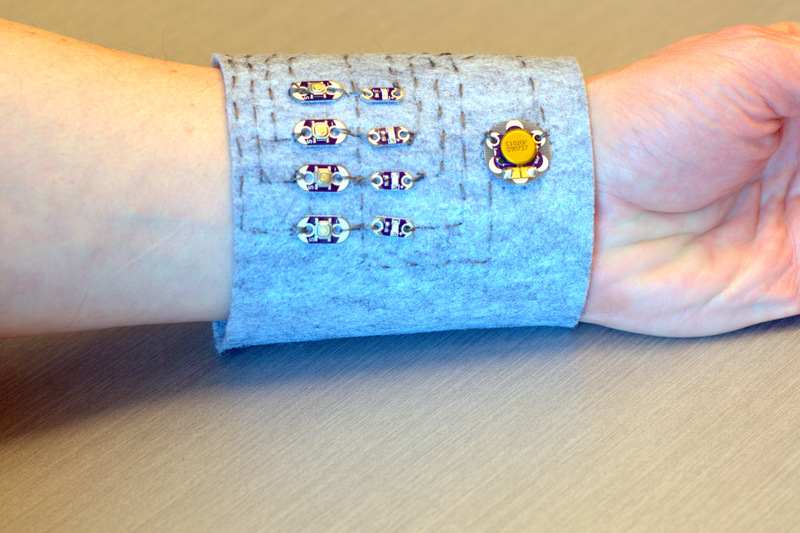
\includegraphics[width=\marginparwidth]{images/P1130375.jpg}
  \caption{A wearable version of the traditional Simon Says game. The wearer repeats flashed visual patterns by pressing buttons adjacent to each LED.}
  \label{fig:simonSays}
  \end{center}  
\end{figure}
}


\marginpar{
\begin{figure}
  \begin{center}
  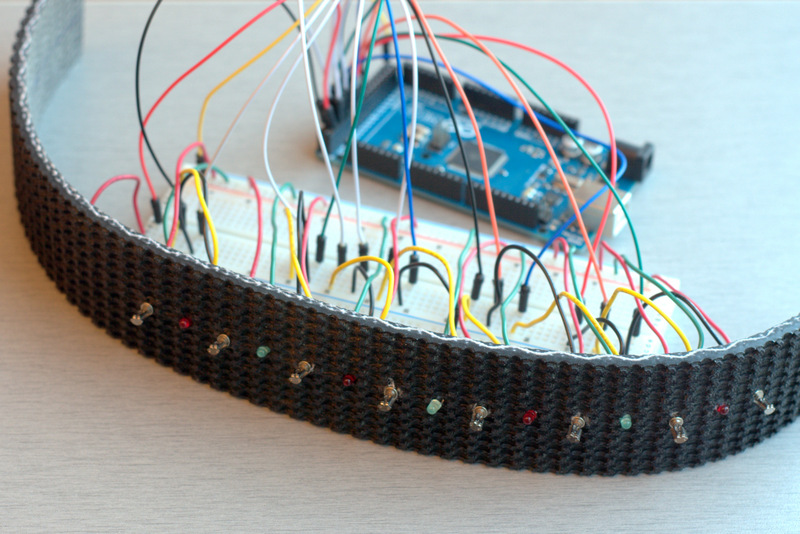
\includegraphics[width=\marginparwidth]{images/P1130394.jpg}
  \caption{A prototype for a wearable that has a simple 1D array of LED light and vibrating motors.}
  \label{fig:rubberBand1}
  \end{center}  
\end{figure}
}

\subsection{Simon Says Wristband}
This is a wearable version of the traditional \emph{Simon Says} game mounted onto a flexible velcro and felt wristband (see Figure~\ref{fig:simonSays}). The game is controlled by four push buttons each with a corresponding LED light. The LEDs flash in a random pattern and a single vibration motor signals the beginning of a new game. To play the game the wearer repeats the pattern as flashed by the LEDs by pressing the buttons directly adjacent to each LED. 

%This wristband's components are:
%\begin{inparaenum}[\itshape a\upshape)]
%\item Felt wristband and Velcro closer
%\item Lilypad Arduino
%\item Push buttons
%\item LEDS (red, blue, yellow, green)
%\item Vibration Motor
%\item Conductive thread
%\item Power supply
%\end{inparaenum}

%\subsection{Screen-based Wrist Wearable}
%This prototype is as yet, not wearable but has a compact OLED screen with a pixel  resolution of 128x128. The intention for this device was to support interactions with a collections and task-based transmedia game called Time Tremors. The screen displays several items of interest for simple task-based games: name of task, efficiency at completing task, time spent on task and visualization of task.
%
%Currently, compact, relatively high resolution screens (for instance, in pixel resolution of 128x128, or 96x96) are compact, inexpensive and provide clear images, which enables high-density information display similar to that found on smartphone and tablet displays, yet in a very compact form factor. This is in contrast to other devices shown here that have very low resolution input and output arrays. High density visual displays requires different types of interactions compared to very low resolution arrays and require operating software quite different from that which low resolution input and output arrays require.
%
%This prototype's components are:
%\begin{inparaenum}[\itshape a\upshape)]
%\item 2200 mAh LiPo battery
%\item 128 x 128 pixel OLED display
%\item 5V step-up for LiPo battery
%\end{inparaenum}
%
%\begin{figure}
%  \begin{center}
%  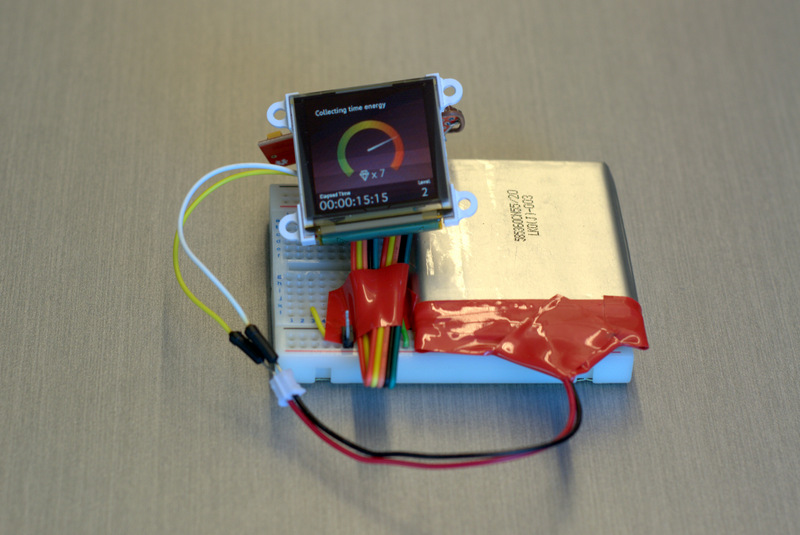
\includegraphics[width=\columnwidth]{images/P1130382.jpg}
%  \caption{A prototype for a wearable that has a compact, yet high resolution OLED screen.}
%  \label{fig:oledscreen}
%  \end{center}  
%\end{figure}

\subsection{Rubber vibration band version 1}
This wrist band with a thick rubber band has vibrating motors and LED lights (see Figure~\ref{fig:rubberBand1}). Vibrating motors and lights are arranged linearly with motors alternating with lights. It connects to and is controlled by an Arduino Mega microcontroller board. The prototype device is thick and unfortunately can't be worn (some components come out the back of the device). The device has no input buttons or other input devices. 

%This wristband's components include	:
%\begin{inparaenum}[\itshape a\upshape)]
%\item 16mm x 6mm mobile phone vibrators (Panasonic)
%\item LED lights (red/green)
%\item rubber band (conveyor belt material)
%\item Arduino Mega 2560 controller board, w/ wired connectors
%\end{inparaenum}



\marginpar{
\begin{figure}
  \begin{center}
  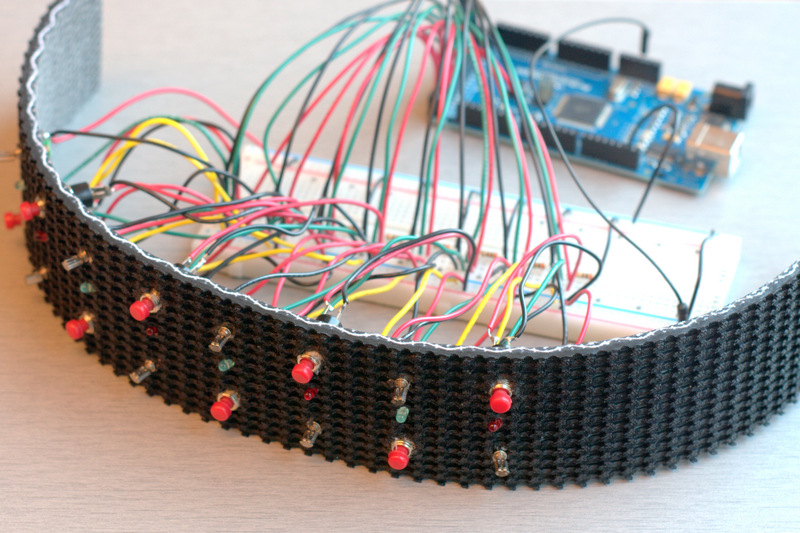
\includegraphics[width=\marginparwidth]{images/P1130396.jpg}
  \caption{A prototype for a wearable that has a 3x8 array of buttons, LED lights and vibrating motors.}
  \label{fig:rubberBand2}
  \end{center}  
\end{figure}
}

\marginpar{
\begin{figure}
  \begin{center}
  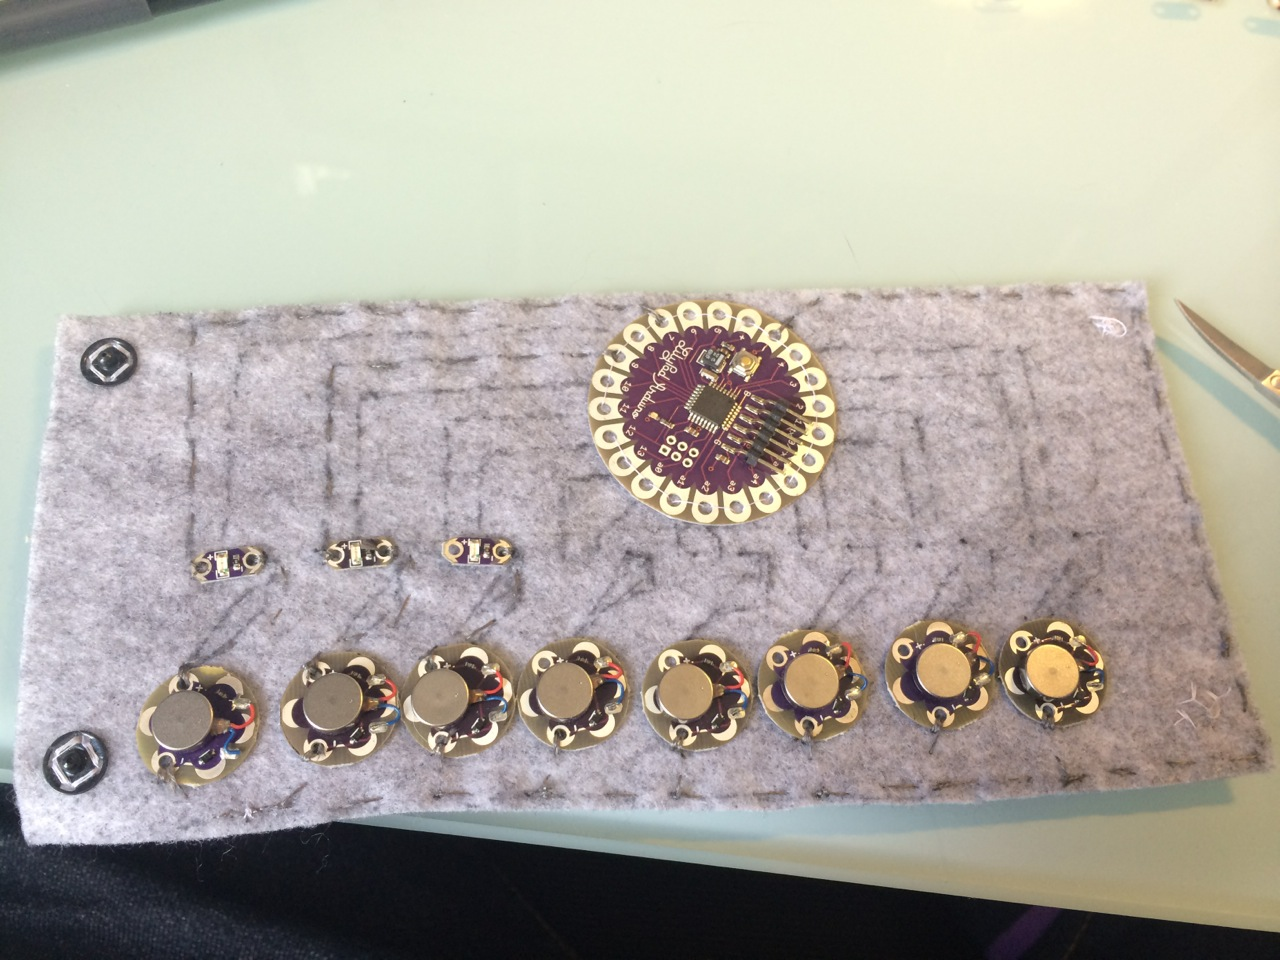
\includegraphics[width=\marginparwidth]{images/IMG_4433.jpeg}
  \caption{Final wearable prototype with 8 tactors with soft buttons and 8 LEDs.}
  \label{fig:felt2}
  \end{center}  
\end{figure}
}
\subsection{Rubber vibration band version 2}
This band is similar to the first band but instead of a linear pattern, there is 3x8 array of buttons, lights, and vibrating motors (see Figure~\ref{fig:rubberBand2}). Each row of this array has one button, one light and one vibrator that are all independent, allowing for the creation of interactive buttons games like \emph{Simon Says}. The 3x8 matrix starts to afford more possibilities for user interaction. Modal play becomes possible since many types of user notifications are possible with such an array. 

\subsection{Wearable Vibrotactile Game Interface}
The final interface (see Figure~\ref{fig:felt2}) utilizes the learnings in the rubber band prototypes, combining visual and tactile feedback, with a form factor that is able to be comfortably worn, like our first prototype. Additionally, the buttons on the final interface are soft buttons that are activated by pressing on the tactors. 

\subsection{Informal User Study}

%This wristband's components include:
%\begin{inparaenum}[\itshape a\upshape)]
%\item 16mm x 6mm mobile phone vibrators (Panasonic)
%\item LED lights (red/green)
%\item rubber band (conveyor belt material)
%\item Arduino Mega 2560 controller board, w/ wired connectors
%\item Push buttons (push on / norm off); Each individual component has its own digital pin on the Arduino board (3x8 = 24 pins in total).
%\end{inparaenum}

%The prototypes consist of simple arrays of vibrating motors and LED lights. Later prototypes add buttons to these components. What patterns can be created when using these components? The simplest are non-directional ones, such as flashing patterns [all on, then all off]. Other simulate movement using 1D and 2D transformations.

%\subsection{Types of Patterns}
%We have found that even the simplest patterns can convey interesting sensations with informational potential. A simple one-dimensional row of LED lights can flash in several different ways: \begin{inparaenum}[\itshape a\upshape)]
%\item it can flash all its LEDs at once
%\item it can flash in a sequential, directional pattern. 
%\item it can vary the intensity of the LEDs in a pulsating pattern
%\item it can illuminate only the red or the green LEDs, and
%\item it can flash its lights in a random pattern. 
%\end{inparaenum}

%\begin{inparaenum}[\itshape a\upshape)]
%\item flashing, non-directional ones in which all the lights or all the vibe motors activate at the same time. These might be useful, for instance, when the gamer has achieved a new level in a game;
%\item flashing, directional ones which there is a sequential activation such that they appear to point in a specific direction. These could be used when the gamer detects another player in the vicinity and the device shows the direction where the other player is located;
%\item flashing, expanding ones where a pattern is generated from a 'point of impact' and expands outwards in 2D, similar to what you might find in the 'Game of Life'
%\end{inparaenum}

%\subsection{Functions for Patterns}
%TBD

%\subsection{Development of prototypes}
%Prototypes began as the simplest and least refined expression of a wearable or functional haptic device. The first prototype has simple linear arrangement of LED light and mobile phone type vibrating motors. When the connected to an Arduino micro-controller this band emits a rhythmic and visual sequential pattern that could conceivably could be used to notify band wearers of others in their vicinity. 

%Although this band was perhaps the most simplistic band possible, it could in fact be functional in some minimal sense for a transmedia gaming experience. Also, such a minimal band would be inexpensive to manufacture and simple to program. 

%Prototypes began as the simplest and least refined expression of a wearable or functional haptic device. The first prototype has simple linear arrangement of LED light and mobile phone type vibrating motors. When the connected to an Arduino micro-controller this band emits a rhythmic and visual sequential pattern that could conceivably could be used to notify band wearers of others in their vicinity. Although this band was perhaps the most simplistic band possible, it could in fact be functional in some minimal sense for a gaming experience. 

%\subsection{Component Patterns vs. Dynamic Interactive Patterns}
%Two types of patterns involved int the devices prototyped: there are the simple grids of the components themselves, and then there are the patterns which can generated using these simple components. When lights and vibrating motors can actuate in a dynamic way, then the dynamics that can be designed, such as flashes, waves and very low resolution visual images, can produce very interesting effects. 

%\subsection{Wearability and Testing}
%These kind of devices at the prototype stage are far from being wearable. They are typically connected to an Arduino board and have bulky components and wired connections that interfere with basic wearability. This makes testing of such devices in a natural context difficult or impossible. A question that arises is how to decide, in an evidence-based manner, which devices to develop further such that they become miniaturized and wearable. 

\section{Future Work}
The resolution of the haptic channel on the wrist in both the spatial and temporal dimensions are not fully studied. The next prototypes will include different sizes of vibrotactile arrays so that we may figure out how many motors are required to maximize the information reception through the tactile channel in the wrist. Specifically, are going to build and test devices that include 6, 4, 2, and 1 vibrating motors. 

In addition to gaming applications, the devices will be used for encoding more critical information and testing the effectiveness of non-gaming contexts with vibrotactile arrays. We are currently developing a method of authoring the vibration sequences so that they may be more effectively created, stored, processed, and shared. 

%One approach to the authoring task is to compose rhythmic sequences as types of musical compositions. The text-based music notation software Lilypond \cite{nienhuys2003lilypond} could be used for this purpose. Output of midi events from composition defined in Lilypond could then up uploaded directly onto Arduino micro-controller boards using the Arduino midi library \cite{best2014arduinoMidi}. Since temporal patterning is the most easily distinguishable parameter for wrist tactile patterns (as noted in \cite{lee2010buzzwear}), it may make sense to involve musical approaches that also deal with the design of temporal patterning.

\section{Conclusion}
Vibrotactile arrays combine with simple visual patterns present new possibilities for information display to users through their body. We have demonstrated the use of a wearable multichannel vibrotactile and visual display intended for gaming in order to explore the uses and affordances in a non-critical usage scenario. 

\section{Acknowledgements}
%We thank the valuable input from Patrick Crowe and all those at Xenophile Media Inc. who have great expertise in crafting transmedia narratives; Dr. Rachel Zuannon from the Graduate Design Program at Anhembi Morumbi University, Sao Paulo, Brazil.; the professors, students and staff within OCAD University's Digital Futures Initiative (DFI) for their valuable input and helpful comments. The following students within the DFI program worked on this project over many months: Hudson Pridham, Ryan Maksymic, Jessica Peter and Boris Kourtoukov. We thank Dr. Steve Szigeti for his contributions to this project and we especially thank Dr. Sara Diamond, President of OCAD University for her guidance and support.

We would like to thank Ryan Maksymic, Boris Kourtoukov, and Steve Szigeti for their help in the development of this project. This work is generously supported by grants from the Natural Sciences and Engineering Research Council of Canada (NSERC), International Science and Technology Partnerships Canada.

\balance
\bibliographystyle{acm-sigchi}
\bibliography{MGDSPET}

\end{document}
